\chapter{Практическая часть}

\section{Задание}

%Условие:
%\begin{itemize}
%\item структурировать исходный код программы в листинге 4.7;
%\item изменить программу так, чтобы она выводила на экран дерево каталогов;
%\item изменить функцию myftw() так, чтобы каждый раз, когда встречается каталог, функции lstat() передавался не полный путь к файлу, а только его
%имя. Для этого после обработки всех файлов в каталоге вызовите chdir(“..”).
%\end{itemize}

Ниже представлен листинг программы.

\lstset{language=c}
\begin{lstlisting}[caption=Текст программы]
#include <sys/stat.h>
#include <sys/types.h>
#include <dirent.h>
#include <limits.h>
#include <stdio.h>
#include <unistd.h>
#include <string.h>
#include <errno.h>
#include <stdarg.h>
#include <stdlib.h>

#define FTW_F 1
#define FTW_D 2
#define FTW_DNR 3
#define FTW_NS 4
#define	MAXLINE	4096

typedef int MyFunc(const char * ,const struct stat *, int);

static MyFunc myfunc;
static int myftw(char *, MyFunc*);
static int dopath(const char* filename, int depth, MyFunc*);

static long nreg, ndir, nblk, nchr, nfifo, nslink, nsock, ntot;

static void err_doit(int errnoflag, int error, const char *fmt, va_list ap);
err_quit(const char *fmt, ...);

int main(int argc, char *argv[])
{
   int ret;

	if (argc != 2)
	{
		err_quit("Usage: ./a.out <start_directory>\n");
	}

   ret = myftw(argv[1], myfunc);

   ntot = nreg + ndir +  nblk + nchr +  nfifo + nslink + nsock;

    if (ntot == 0)
		ntot = 1;

	printf("-------------------------------\n\n");
	printf("Regular files:\t%7ld, %5.2f %%\n", nreg, nreg*100.0/ntot);
	printf("Catalogs:\t%7ld, %5.2f %%\n", ndir, ndir*100.0/ntot);
	printf("Block-devices:\t%7ld, %5.2f %%\n", nblk, nblk*100.0/ntot);
	printf("Char-devices:\t%7ld, %5.2f %%\n", nchr, nchr*100.0/ntot);
	printf("FIFOs:\t\t%7ld, %5.2f %%\n", nfifo, nfifo*100.0/ntot);
	printf("Sym-links:\t%7ld, %5.2f %%\n", nslink, nslink*100.0/ntot);
	printf("Sockets:\t%7ld, %5.2f %%\n\n", nsock, nsock*100.0/ntot);
    printf("Total:\t%7ld\n", ntot);

    exit(ret);
}

static void err_doit(int errnoflag, int error, const char *fmt, va_list ap)
{
	char buf[MAXLINE];

	vsnprintf(buf, MAXLINE-1, fmt, ap);
	if (errnoflag)
		snprintf(buf+strlen(buf), MAXLINE-strlen(buf)-1, ": %s",
		  strerror(error));
	strcat(buf, "\n");
	fflush(stdout);		/* in case stdout and stderr are the same */
	fputs(buf, stderr);
	fflush(NULL);		/* flushes all stdio output streams */
}
err_quit(const char *fmt, ...)
{
	va_list ap;

	va_start(ap, fmt);
	err_doit(0, 0, fmt, ap);
	va_end(ap);
	exit(1);
}

static int myftw(char * pathname, MyFunc *func)
{
    return(dopath(pathname, 0, func));
}

static int dopath(const char* filename, int depth, MyFunc * func)
{
    struct stat statbuf;
    struct dirent * dirp;
    DIR * dp;
    int ret = 0;

    if (lstat(filename, &statbuf) < 0)
        return(func(filename, &statbuf, FTW_NS));

    for (int i = 0; i < depth; ++i)
		printf("|\t");

    if (S_ISDIR(statbuf.st_mode) == 0)
        return(func(filename, &statbuf, FTW_F));

    if ((ret = func(filename, &statbuf, FTW_D)) != 0)
        return(ret);

    if ((dp = opendir(filename)) == NULL)
        return(func(filename, &statbuf, FTW_DNR));

    chdir(filename);
    while ((dirp = readdir(dp)) != NULL && ret == 0)
    {
        if (strcmp(dirp->d_name, ".") != 0 &&
            strcmp(dirp->d_name, "..") != 0 )
        {
            ret = dopath(dirp->d_name, depth+1, func);
        }
    }

    chdir("..");

    if (closedir(dp) < 0)
        perror("Unable to close directory");

    return(ret);
}

static int myfunc(const char* pathame, const struct stat * statptr, int type)
{
    switch(type)
    {
        case FTW_F:
            printf( "-- %s\n", pathame);
            switch(statptr->st_mode & S_IFMT)
            {
                case S_IFREG: nreg++; break;
                case S_IFBLK: nblk++; break;
                case S_IFCHR: nchr++; break;
                case S_IFIFO: nfifo++; break;
                case S_IFLNK: nslink++; break;
                case S_IFSOCK: nsock++; break;
                case S_IFDIR:
                    perror("The directory is of type FTW_F"); return(-1);
            }
            break;
        case FTW_D:
            printf( "-- %s/\n", pathame);
            ndir++; break;
        case FTW_DNR:
            perror("Blocked access to one of the directories!"); return(-1);
        case FTW_NS:
            perror("Function error stat!"); return(-1);
        default:
            perror("Unknown file type!"); return(-1);
    }

    return(0);
}
\end{lstlisting}

\newpage

\section{Результат}

Демонстрация запуска программы с неправильными аргументами:
\begin{figure}[H]
    \centering
    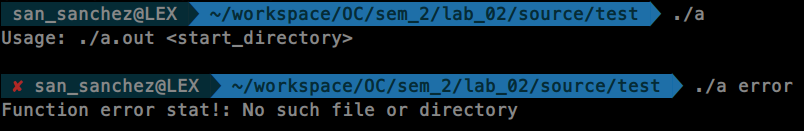
\includegraphics[scale=0.5]{data/image/error.png}
    \caption{Скришот запуска программы.}
\end{figure}

Демонстрация корректного запуска программы:
\begin{figure}[H]
    \centering
    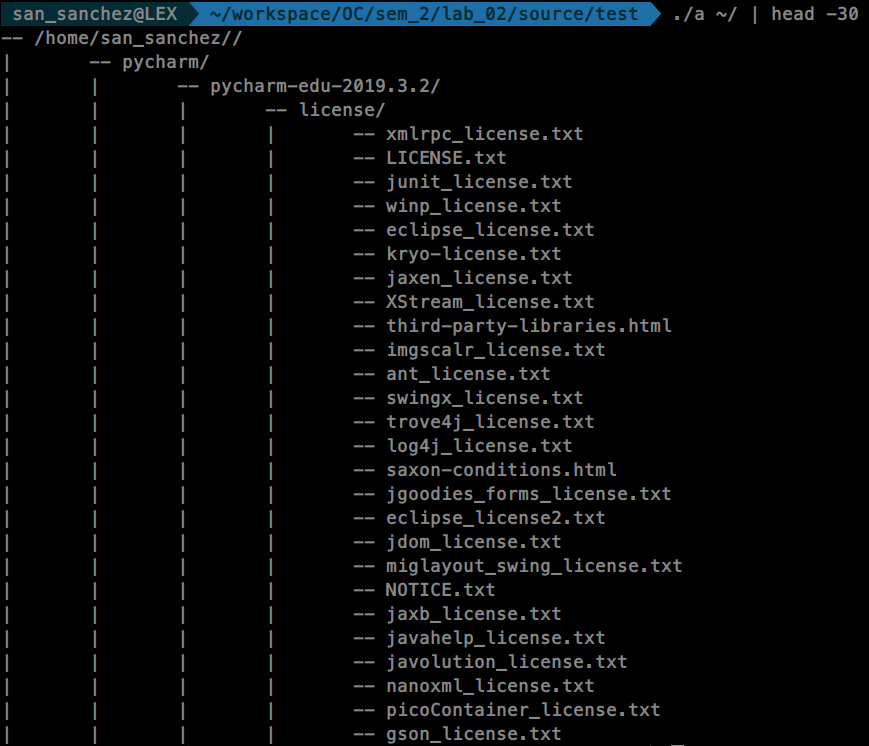
\includegraphics[scale=0.5]{data/image/work_1.png}
    \caption{Скришот вывода программы.}
\end{figure}

\begin{figure}[H]
    \centering
    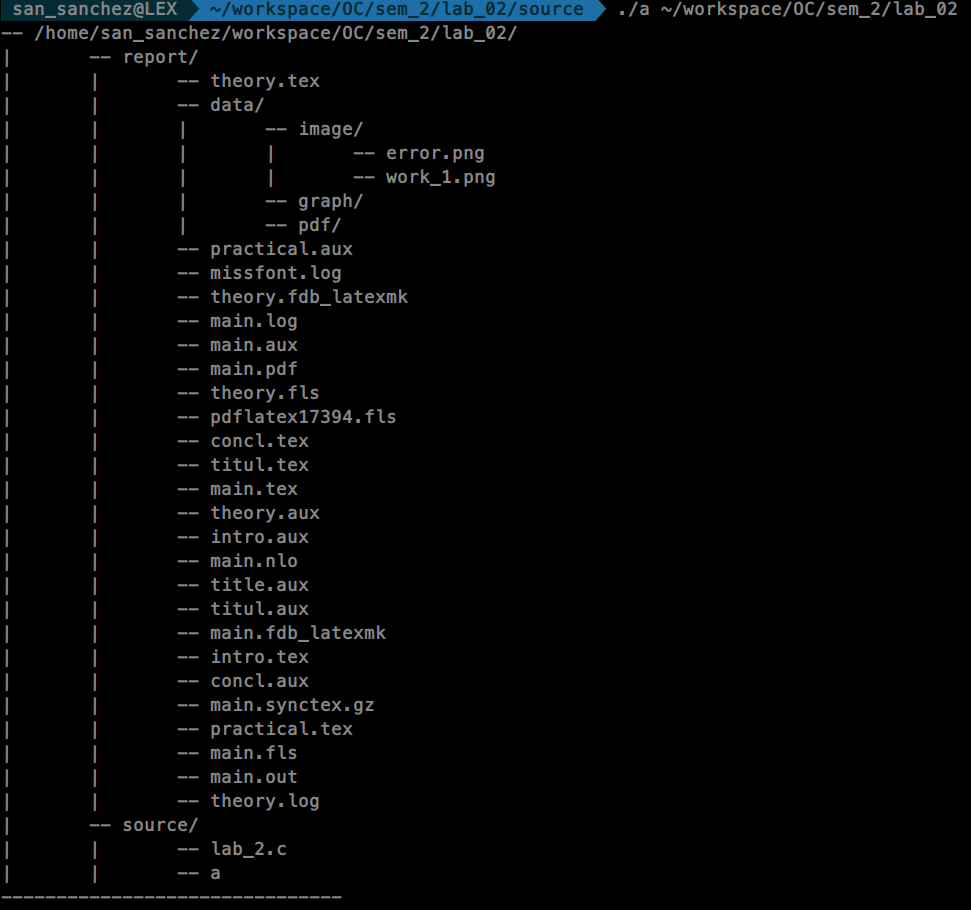
\includegraphics[scale=0.5]{data/image/work_2.png}
    \caption{Скришот результата работы программы (часть 1).}
\end{figure}
\begin{figure}[H]
    \centering
    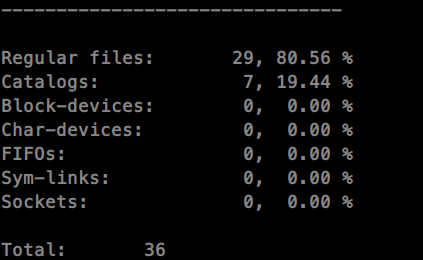
\includegraphics[scale=0.6]{data/image/work_3.png}
    \caption{Скришот результата работы программы (часть 2).}
\end{figure}



